\documentclass[tikz,border=10pt]{standalone}
\usepackage{amsmath,amssymb}
\usetikzlibrary{arrows.meta,calc,positioning}
\definecolor{TargetBlue}{HTML}{2364AA}
\definecolor{NuisanceOrange}{HTML}{E6862A}
\definecolor{EfficientGreen}{HTML}{278A64}
\definecolor{NeutralGray}{HTML}{68717C}
\definecolor{Ink}{HTML}{18212B}
\begin{document}
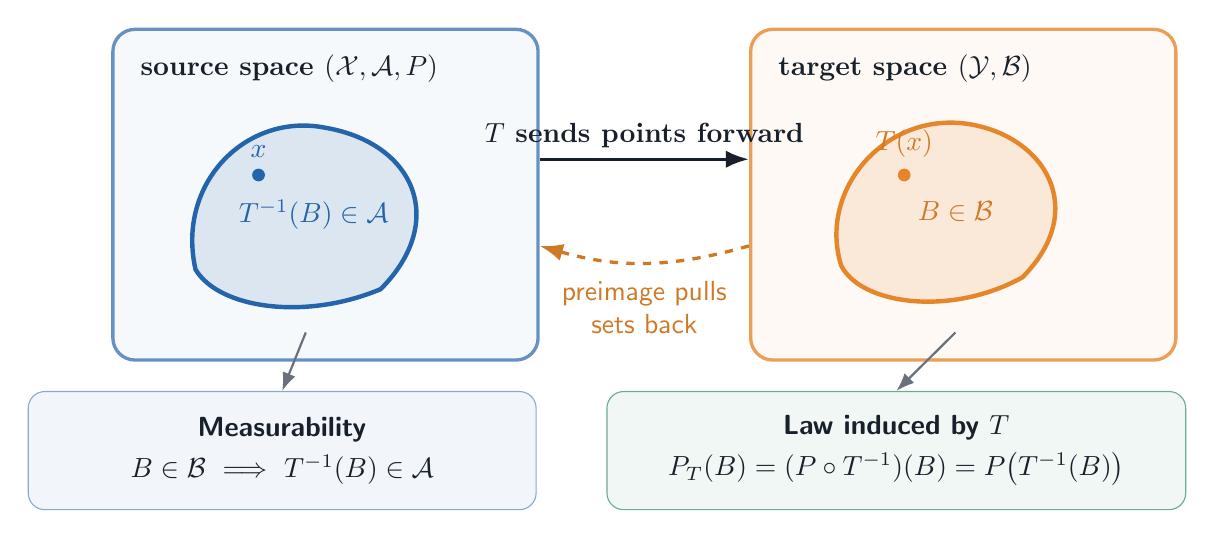
\begin{tikzpicture}[font=\sffamily, >=Latex]
  % The two measurable spaces.
  \node[draw=TargetBlue!70, very thick, rounded corners=8pt,
    fill=TargetBlue!4, minimum width=5.4cm, minimum height=4.2cm] (source) at (0,0) {};
  \node[draw=NuisanceOrange!80, very thick, rounded corners=8pt,
    fill=NuisanceOrange!5, minimum width=5.4cm, minimum height=4.2cm] (target) at (8.1,0) {};
  \node[anchor=north west, text=Ink, font=\bfseries] at ($(source.north west)+(0.25,-0.22)$)
    {source space $(\mathcal X,\mathcal A,P)$};
  \node[anchor=north west, text=Ink, font=\bfseries] at ($(target.north west)+(0.25,-0.22)$)
    {target space $(\mathcal Y,\mathcal B)$};

  % A target set and its preimage.
  \draw[TargetBlue, ultra thick, fill=TargetBlue!16]
    (-1.65,-0.95) .. controls (-1.9,0.15) and (-1.0,1.05) .. (0.0,0.85)
    .. controls (1.15,0.65) and (1.55,-0.35) .. (0.7,-1.2)
    .. controls (-0.25,-1.6) and (-1.35,-1.45) .. cycle;
  \node[text=TargetBlue, font=\bfseries] at (-0.15,-0.25) {$T^{-1}(B)\in\mathcal A$};

  \draw[NuisanceOrange, ultra thick, fill=NuisanceOrange!18]
    (6.55,-0.9) .. controls (6.25,0.05) and (7.1,1.05) .. (8.15,0.9)
    .. controls (9.15,0.75) and (9.7,-0.2) .. (8.85,-1.05)
    .. controls (7.95,-1.55) and (6.8,-1.4) .. cycle;
  \node[text=NuisanceOrange!90!black, font=\bfseries] at (8.0,-0.22) {$B\in\mathcal B$};

  % Pointwise map and setwise pullback.
  \coordinate (x) at (-0.85,0.25);
  \coordinate (Tx) at (7.35,0.25);
  \fill[TargetBlue] (x) circle (2.3pt);
  \fill[NuisanceOrange] (Tx) circle (2.3pt);
  \node[above=1mm of x, text=TargetBlue] {$x$};
  \node[above=1mm of Tx, text=NuisanceOrange!90!black] {$T(x)$};
  \draw[->, very thick, text=Ink, draw=Ink] ($(source.east)+(0,0.45)$) --
    node[above, font=\bfseries] {$T$ sends points forward}
    ($(target.west)+(0,0.45)$);
  \draw[->, dashed, very thick, NuisanceOrange!90!black]
    ($(target.west)+(0,-0.65)$) to[bend left=16]
    node[below=1mm, align=center] {preimage pulls\\sets back}
    ($(source.east)+(0,-0.65)$);

  % Two consequences of the same preimage operation.
  \node[draw=TargetBlue!55, fill=TargetBlue!6, rounded corners=6pt,
    minimum width=6.45cm, minimum height=1.5cm, align=center, text=Ink]
    (measurable) at (-0.55,-3.25)
    {\textbf{Measurability}\\[1mm]
     $B\in\mathcal B\ \Longrightarrow\ T^{-1}(B)\in\mathcal A$};
  \node[draw=EfficientGreen!70, fill=EfficientGreen!7, rounded corners=6pt,
    minimum width=7.35cm, minimum height=1.5cm, align=center, text=Ink]
    (law) at (7.25,-3.25)
    {\textbf{Law induced by $T$}\\[1mm]
     $P_T(B)=(P\circ T^{-1})(B)=P\!\left(T^{-1}(B)\right)$};

  \draw[->, NeutralGray, thick] (-0.25,-1.75) -- (measurable.north);
  \draw[->, NeutralGray, thick] (8.0,-1.75) -- (law.north);
\end{tikzpicture}
\end{document}
